\ifx\wholebook\relax \else

\documentclass[b5paper]{article}
\usepackage[nomarginpar
  %, margin=.5in
]{geometry}

\addtolength{\oddsidemargin}{-0.05in}
\addtolength{\evensidemargin}{-0.05in}
\addtolength{\textwidth}{0.1in}
\usepackage[en]{../../../prelude}

\setcounter{page}{1}

\begin{document}

\title{B-Tree}

\author{Xinyu LIU
\thanks{{\bfseries Xinyu LIU} \newline
  Email: liuxinyu95@gmail.com \newline}
  }

\maketitle
\fi

\markboth{B-Tree}{Elementary Algorithms}

\ifx\wholebook\relax
\chapter{B-Tree}
\numberwithin{Exercise}{chapter}
\fi

\section{Introduction}
\index{B-tree}
\label{introduction}

In previous chapter when develop integer prefix tree, we encode the information in the edge of the binary tree. Another way to extend the binary search tree is to increase the number of the sub-trees from 2 to $k$. B-tree is such a data structure, that can be considered as a generic form of $k$-ary search tree. It is also developed to be self-balanced\cite{wiki-b-tree}. B-tree is widely used in computer file system (some are based on B+ trees, an extension of B-tree) and database system. Figure \ref{fig:btree-example} gives an example B-tree, we can find the differences and similarities between B-tree and binary search tree.

\begin{figure}[htbp]
  \centering
  \includegraphics[scale=0.5]{img/btree-example.ps}
  \caption{A B-Tree}
  \label{fig:btree-example}
\end{figure}

A binary search tree is either empty or a node containing a key $k$ and two sub-trees $l$ and $r$. Every key in $l$ is less than $k$, while $k$ is less than every key in $r$:

\be
\forall\ x \in l, y \in r \Rightarrow x < k < y
\ee

Extend it to multiple keys and sub-trees, we obtain the B-tree. A B-tree is either empty or contains $n$ keys, and $n + 1$ sub-trees, each sub-tree is also a B-Tree. We denote these keys and sub-trees as $k_1, k_2, ..., k_n$ and $t_1, t_2, ..., t_n, t_{n+1}$, as shown in figure \ref{fig:btree-node}.

\begin{figure}[htbp]
  \centering
  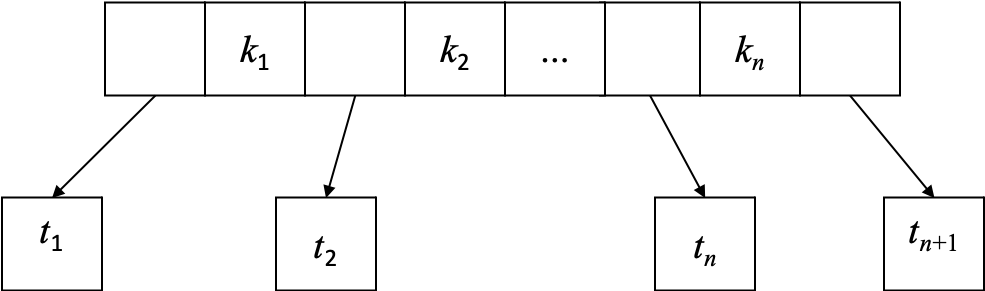
\includegraphics[scale=0.5]{img/btree-node.png}
  \caption{A B-Tree node}
  \label{fig:btree-node}
\end{figure}

For every node, the keys and sub-trees satisfy the following ordering:

\begin{itemize}
\item Keys are in ascending order, that $k_1 < k_2 < ... < k_n$;
\item For every key $k_i$, all keys in sub-tree $t_i$ are less than it, while $k_i$ is less than every keys in sub-tree $t_{i+1}$:
\end{itemize}

\begin{equation}
\forall\ x_i \in t_i, i=0, 1, ..., n, \Rightarrow x_1 < k_1 < x_2 < k_2 < ... < x_n < k_n < x_{n+1}
\label{eq:btree-order}
\end{equation}

For leaf node, there is no sub-trees. There can be optional values bound to keys in B-tree node. We skip the values for simplicity, and denote the B-tree of keys in type $K$ as $BTree\ K$, or \texttt{BTree<K>}. On top of it, we also need define a set of self-balance rules:

\begin{enumerate}
\item All leaves have the same depth;
\item Let $d$ be the {\em minimum degree} number of a B-tree, such that each node:
  \begin{itemize}
  \item has at most $2d - 1$ keys;
  \item has at least $d - 1$ keys, except for the root;
  \end{itemize}
\end{enumerate}

\be
  d - 1 \leq |keys(t)|  \leq 2d - 1
\ee

\begin{proof}
Let's prove that a B-tree is always balanced. Consider a B-tree of $n$ keys. The minimum degree $d \geq 2$. Let the height be $h$. All the nodes have at least $d - 1$ keys except for the root. The root contains at least 1 key. There are at least 2 nodes at depth 1, at least $2d$ nodes at depth 2, at least $2d^2$ nodes at depth 3, ..., at least $2d^{h-1}$ nodes at depth $h$. Multiply all nodes with $d-1$ except for the root, the total number of keys satisfies the following:

\be
\begin{array}{rl}
n & \geq 1 + (d - 1)(2 + 2d + 2d^2 + ... + 2d^{h-1}) \\
  & = 1 + 2(d - 1) \displaystyle \sum_{k=0}^{h-1} d^k \\
  & = 1 + 2(d - 1) \displaystyle \frac{d^h-1}{d-1} \\
  & = 2d^h - 1
\end{array}
\ee

It limits the tree height with logarithm of the number of keys.

\be
h \leq \log_d \frac{n+1}{2}
\ee

\end{proof}

Hence B-tree is balanced. The simplest B-tree is called 2-3-4 tree, where $d = 2$. Every node except for the root contains 2, 3, or 4 sub-trees. Essentially, a red-black tree can be mapped to a 2-3-4 tree. For a none empty B-tree of degree $d$, we denote it as $(d, (ks, ts))$, where $ks$ is the keys, $ts$ is the sub-trees. Below example program defines the B-tree.

\lstset{frame = single}
\begin{Haskell}
data BTree a = BTree { keys :: [a]
                     , subTrees :: [BTree a] }
\end{Haskell}

The empty node is in the form of $(\nil, \nil)$ or \texttt{BTree [] []}. Instead of storing $d$ in every node, we pass it together with B-tree $t$ as a pair $(d, t)$.

\section{Insert}
\label{btree-insertion} \index{B-tree!insert}

The idea of B-tree insertion is similar to the binary search tree. The difference is we need deal with multiple keys and sub-trees. When insert key $x$ to a B-tree $t$, start from the root, we examine the keys in the node to locate a position where all keys on the left to this position are less than $x$, while the rest keys on the right are greater than $x$.\footnote{In fact, only less-than and equality are sufficient. See exercise after this section.} If the node is a leaf, and is not full ($|keys(t)| < 2d-1$), we insert $x$ at this position. Otherwise, this position points to a sub-tree $t'$, we recursively insert $x$ to $t'$.

\begin{figure}[htbp]
  \centering
  \subcaptionbox{Insert 22 to a 2-3-4 tree. $22 > 20$, go to the right sub-tree; next as $22 < 26$, go to the first sub-tree.}{\includegraphics[scale=0.5]{img/btree-insert-simple1.ps}} \\
  \subcaptionbox{$21 < 22 < 25$, the leaf is not full.}{\includegraphics[scale=0.5]{img/btree-insert-simple2.ps}}
  \caption{Insert.} \label{fig:btree-insert-simple}
\end{figure}

As an example, consider the 2-3-4 tree in figure \ref{fig:btree-insert-simple}. when insert $x = 22$, because $20 < 22$, we next examine the sub-tree on the left, which contains 26, 38, 45. Since $22 < 26$, we next go to the first sub-tree containing 21 and 25. This is a leaf, and it is not full. Hence we insert 22 to this node.

However, if there are $2d - 1$ keys in the leaf, we will break the B-tree rules after insert $x$, as the node will be too 'full'. For the same B-tree in figure \ref{fig:btree-insert-simple}, we'll meet this issue when insert 18. There are 2 approaches to solve it.

\subsection{Insert then split}

We can adopt the similar insert then fix method as for red-black tree. First, we insert the key to proper ordering position without considering the B-tree balance rules, then as the next step, if the new tree violates the balance rule, we perform a recursive bottom-up fixing by splitting the overly full nodes. We need define the function to test whether a given node exceeds the minimum degree constraint or not.


\be
\begin{cases}
full\ d\ (ks, ts) & = |ks| > 2d - 1 \\
low\  d\ (ks, ts) & = |ks| < d - 1 \\
\end{cases}
\ee

When the node contains too many keys and sub-trees, we define $split$ function to break it into 3 parts at a given position $m$ as shown in figure \ref{fig:node-split}:

\begin{figure}[htbp]
  \centering
  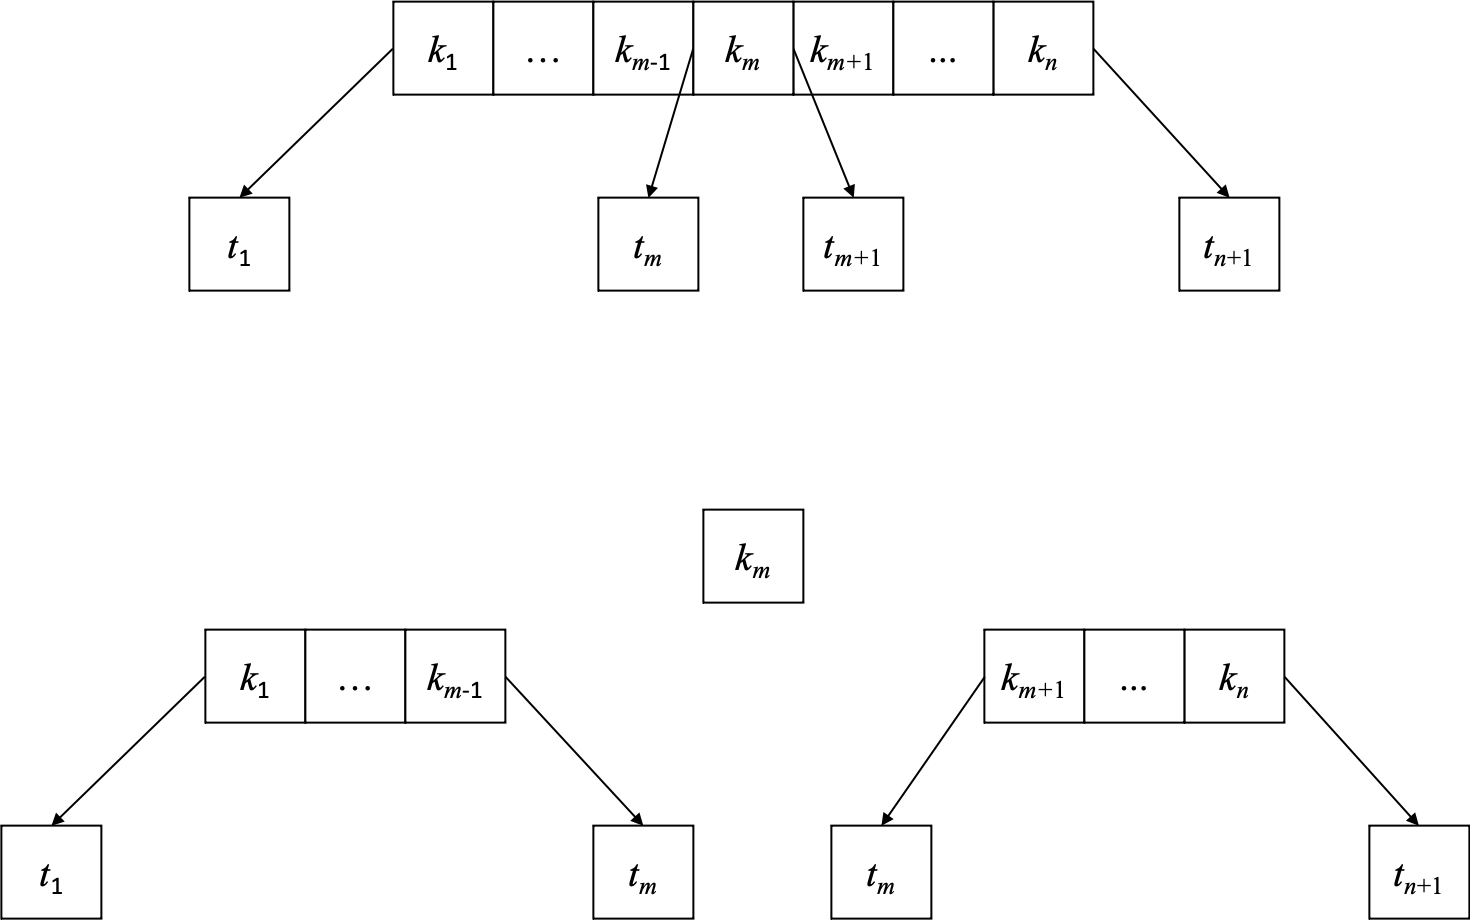
\includegraphics[scale=0.4]{img/split.png}
  \caption{Split the node into 3 parts at $m$}
  \label{fig:node-split}
\end{figure}

\be
split\ m\ (ks, ts) = ((ks_l, ts_l), k, (ks_r, ts_r))
\ee

We can reuse the list $splitAt$ function defined in chapter 1 (\autoref{eq:split-at}) to realize it.

\[
\begin{cases}
(ks_l, (k:ks_r)) & = splitAt\ (m - 1)\ ks \\
(ts_l, ts_r) & = splitAt\ m\ ts
\end{cases}
\]

We can define the reversed operation $unsplit$ to combine the 3 parts back into a B-tree node.

\be
unsplit\ (ks_l, ts_l)\ k\ (ks_r, ts_r) = (ks_l \doubleplus [k] \doubleplus ks_r, ts_l \doubleplus ts_r)
\ee

Below function first insert $x$ to the tree $t$, then call $fix$ to resume the B-tree balance rules with the given degree $d$.

\be
insert\ x\ (d, t) = fix\ (d, ins\ t)
\ee

After $ins$, if the root contains too many keys, function $fix$ calls $split$ to break it and build a new root.

\be
fix\ (d, t) = \begin{cases}
  full\ d\ t : & (d, ([k], [l, r])), \text{where}\ (l, k, r) = split\ d\ t \\
  otherwise  : & (d, t)
\end{cases}
\ee

$ins$ need handle two cases: for leaf node, we can reuse the list ordered $insert$ function defined in chapter 1 (\autoref{eq:list-ordered-insert}); otherwise, we need find the position to recursively insert to sub-tree. To do that, we define a function as: $partition\ x\ (ks, ts) = (l, t', r)$, where $l = (ks_l, ts_l)$ and $r = (ks_r, ts_r)$. It further uses the list partition function $span$ defined in chapter 1 (\autoref{eq:span}):

\[
\begin{cases}
(ks_l, ks_r) & = span\ (< x)\ ks \\
(ts_l, (t':ts_r)) & = splitAt\ |ks_l| ts
\end{cases}
\]

As such, we separate all the keys and sub-trees less than $x$ on the left as $l$, and those greater than $x$ on the right as $r$. The last sub-tree that less than $x$ is extracted as $t'$. We then recursively insert $x$ to $t'$, as shown in figure \ref{fig:recursive-insert}.

\be
\begin{array}{rcll}
  ins\ (ks, \nil) & = & (insert_L\ x\ ks, \nil) & \text{list insert for leaf}\\
  ins\ (ks, ts)   & = & balance\ d\ l\ (ins\ t')\ r & \text{where}\ (l, t', r) = partition\ x\ t \\
\end{array}
\ee

\begin{figure}[htbp]
  \centering
  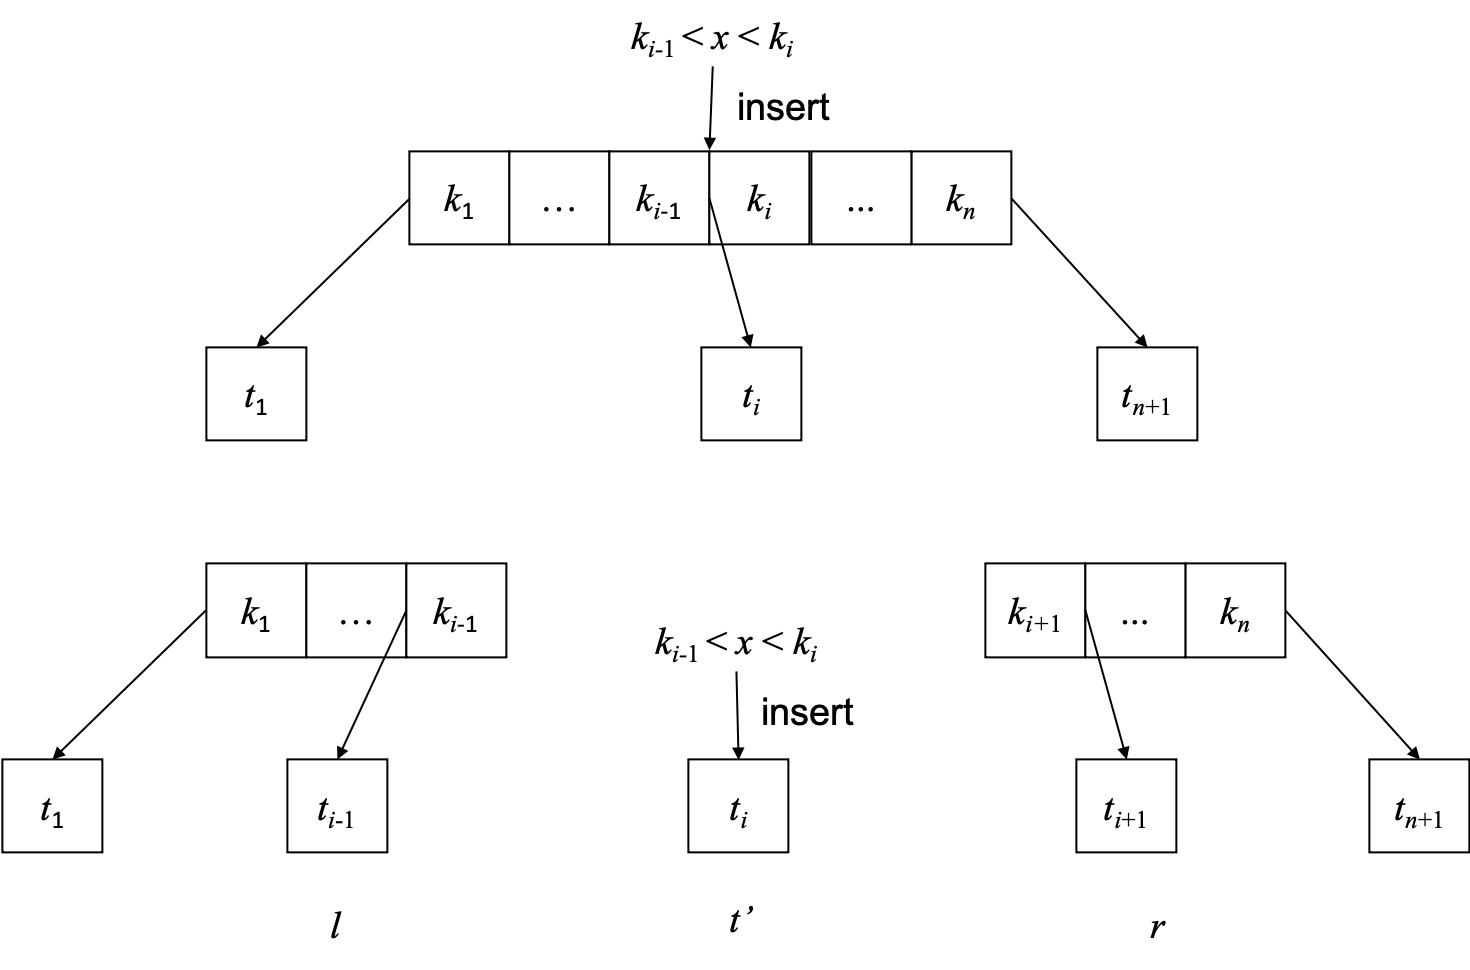
\includegraphics[scale=0.45]{img/partition.png}
  \caption{partition a node with $x$}
  \label{fig:recursive-insert}
\end{figure}

After insert $x$ to $t'$, it may contains too many keys over B-tree constraint. We define function $balance$ to recursively resume B-tree property by splitting sub-tree.

\be
balance\ d\ (ks_l, ts_l)\ t\ (ks_r, ts_r) = \begin{cases}
  full\ d\ t: fix_f \\
  otherwise: ((ks_l \doubleplus ks_r), (ts_l \doubleplus [t] \doubleplus ts_r))
  \end{cases}
\ee

where $fix_f$ splits sub-tree $t$ with degree $d$ as $(t_1, k, t_2) = split\ d\ t$, then combine to a new B-tree node:

\be
fix_f = ((ks_l \doubleplus [k] \doubleplus ks_r), (ts_l \doubleplus [t_1, t_2] \doubleplus ts_r))
\ee

The following example program implements $insert$ for B-tree.

\begin{Haskell}
partition x (BTree ks ts) = (l, t, r) where
  l = (ks1, ts1)
  r = (ks2, ts2)
  (ks1, ks2) = span (< x) ks
  (ts1, (t:ts2)) = splitAt (length ks1) ts

split d (BTree ks ts) = (BTree ks1 ts1, k, BTree ks2 ts2) where
  (ks1, k:ks2) = splitAt (d - 1) ks
  (ts1, ts2) = splitAt d ts

insert x (d, t) = fixRoot (d, ins t) where
    ins (BTree ks []) = BTree (List.insert x ks) []
    ins t = balance d l (ins t') r where (l, t', r) = partition x t

fixRoot (d, t) | full d t  = let (t1, k, t2) = split d t in
                               (d, BTree [k] [t1, t2])
               | otherwise = (d, t)

balance d (ks1, ts1) t (ks2, ts2)
    | full d t  = fixFull
    | otherwise = BTree (ks1 ++ ks2) (ts1 ++ [t] ++ ts2)
  where
    fixFull = let (t1, k, t2) = split d t in
                BTree (ks1 ++ [k] ++ ks2) (ts1 ++ [t1, t2] ++ ts2)
\end{Haskell}

Figure \ref{fig:btree-insert-fp} shows the example B-trees built by repeatedly insert elements from list ``GMPXACDEJKNORSTUVYZ''.

\begin{figure}[htbp]
  \centering
  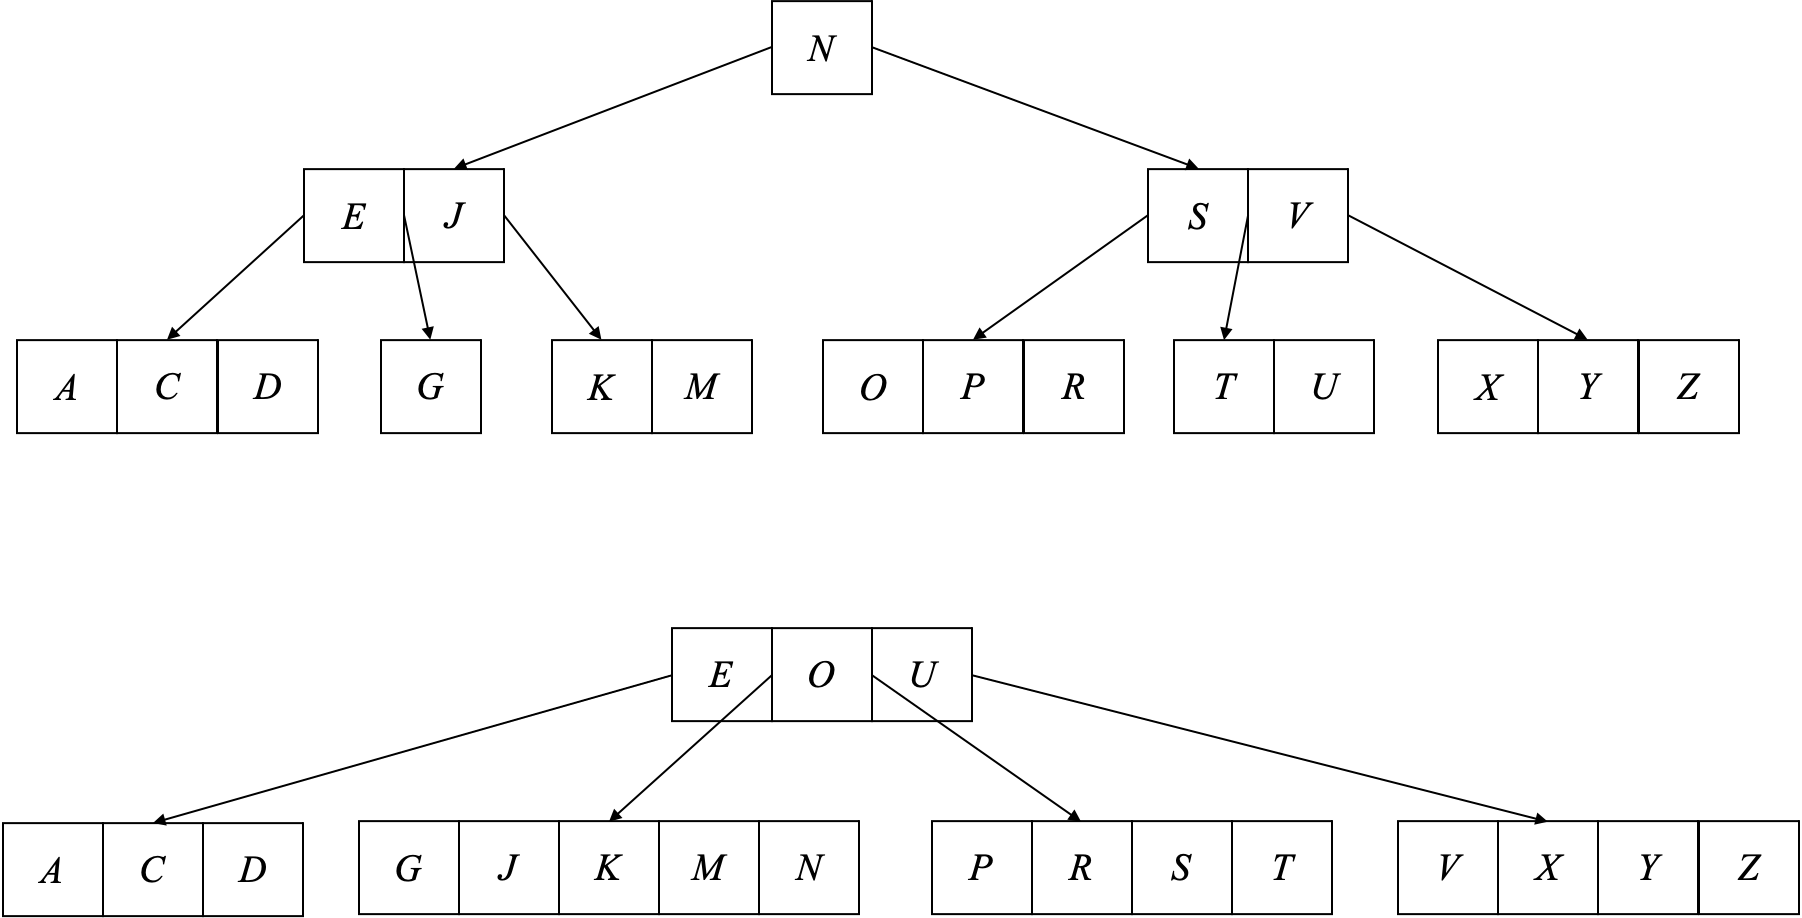
\includegraphics[scale=0.4]{img/btree-insert-fp.png}
  \caption{Repeatedly insert elements from "GMPXACDEJKNORSTUVYZ". above: $d = 2$ (2-3-4 tree), below: $d = 3$}
  \label{fig:btree-insert-fp}
\end{figure}

\subsection{Split before insertion}

The second method is to split a node before insertion to prevent it becoming overly full. We can often see this method in imperative implementations. When perform top-down recursive insert, if we reach to a node with $2d - 1$ keys, we divide it into 3 parts as shown in figure \ref{fig:node-split}, such that each new node has $d - 1$ keys. They will be valid B-tree node after insertion. For node $x$, let $K(x)$ be the keys, $T(x)$ be the sub-trees. Denote the $i$-th key of $x$ as $k_i(x)$, the $j$-th sub-tree as $t_j(x)$. Below algorithm splits the $i$-th sub-tree of node $z$:

\begin{algorithmic}[1]
\Procedure{Split}{$z, i$}
  \State $d \gets$ \Call{Deg}{$z$}
  \State $x \gets t_i(z)$
  \State $y \gets$ \Call{Create-Node}{}
  \State $K(y) \gets [k_{d + 1}(x), k_{d + 2}(x), ..., k_{2d - 1}(x)]$
  \State $K(x) \gets [k_1(x), k_2(x), ..., k_{d-1}(x)]$
  \If{$x$ is not leaf}
    \State $T(y) \gets [t_{d + 1}(x), t_{d + 2}(x), ..., t_{2d}(x)]$
    \State $T(x) \gets [t_1(x), t_2(x), ..., t_d(x)]$
  \EndIf
  \State \Call{Insert-At}{$K(z), i, k_d(x)$}
  \State \Call{Insert-At}{$T(z), i + 1, y$}
\EndProcedure
\end{algorithmic}

When split the node $x = t_i(z)$, we push the $d$-th key $k_d(x)$ up to the parent node $z$. If $z$ is already full, the pushing will broken B-tree rules. To solve this problem, we need do the top-down check from the root along the path when insert. Split any node with $2d - 1$ keys. Since all parent nodes are processed to be not full, they can accept the additional key pushed up. This method needs one single pass down the tree without any back-tracking. If the root is full, we create a new node, and put the root as it singleton sub-tree. Below is the insert algorithm:

\begin{algorithmic}[1]
\Function{Insert}{$t, k$}
  \State $r \gets t$
  \If{$r$ is full} \Comment{root is full}
    \State $s \gets$ \Call{CREATE-NODE}{}
    \State $T(s) \gets [ r ]$
    \State \Call{Split}{$s, 1$}
    \State $r \gets s$
  \EndIf
  \State \Return \Call{Insert-Nonfull}{$r, k$}
\EndFunction
\end{algorithmic}

Where \textproc{Insert-Nonfull} assumes the node $r$ passed in
is not full. If $r$ is a leaf, we insert $k$ to the keys based on order; otherwise, we locate the position, where $k_i(r) < k < k_{i+1}(r)$. Split the sub-tree $t_i(r)$ if it is full, and go on insert to this sub-tree.

\begin{algorithmic}[1]
\Function{Insert-Nonfull}{$r, k$}
  \State $n \gets |K(r)|$
  \If{$r$ is leaf}
    \State $i \gets 1$
    \While{$i \leq n$ and $k > k_i(r)$}
      \State $i \gets i + 1$
    \EndWhile
    \State \Call{Insert-At}{$K(r), i, k$}
  \Else
    \State $i \gets n$
    \While{$i > 1$ and $k < k_i(r)$}
      \State $i \gets i - 1$
    \EndWhile
    \If{$t_i(r)$ is full}
      \State \Call{Split}{$r, i$}
      \If{$k > k_i(r)$}
        \State $i \gets i + 1$
      \EndIf
    \EndIf
    \State \Call{Insert-Nonfull}{$t_i(r), k$}
  \EndIf
  \State \Return $r$
\EndFunction
\end{algorithmic}

This is recursive algorithm is recursive. There is an exercise problem to eliminate the recursion with pure loops. Figure \ref{fig:btree-insert} gives the result with the same input of ``GMPXACDEJKNORSTUVYZ''.

\begin{figure}[htbp]
  \centering
  \subcaptionbox{$d = 2$, 2-3-4 tree}{\includegraphics[scale=0.5]{img/btree-insert-2-3-4.ps}}\\
  \subcaptionbox{$d = 3$}{\includegraphics[scale=0.5]{img/btree-insert-3.ps}}
  \caption{Insert from ``GMPXACDEJKNORSTUVYZ''}
  \label{fig:btree-insert}
\end{figure}

% ================================================================
%               Deletion
% ================================================================
\section{Deletion}
\index{B-tree!delete}

Deleting a key from
B-tree may violate balance properties. Except the root, a node shouldn't
contain too few keys less than $t-1$, where $t$ is the
minimum degree.

Similar to the approaches for insertion, we can either do some preparation
so that the node from where the key being deleted contains enough
keys; or do some fixing after the deletion if the node has too few keys.


% ================================================================
%               Merge before delete method
% ================================================================
\subsection{Merge before delete method}

We start from the easiest case. If the key $k$ to be deleted
can be located in node $x$, and $x$ is a leaf node,
we can directly remove $k$ from $x$. If $x$ is the root (the only
node of the tree), we needn't worry about there are too few
keys after deletion. This case is named as case 1 later.

In most cases, we start from the root, along a path to locate
where is the node contains $k$. If $k$ can be located in the
internal node $x$, there are three sub cases.

\begin{itemize}
\item Case 2a, If the child $y$ precedes $k$ contains enough keys (more than $t$),
we replace $k$ in node $x$ with $k'$, which is
the predecessor of $k$ in child $y$. And recursively remove $k'$
from $y$.

The predecessor of $k$ can be easily located as the last key of child
$y$.

This is shown in figure \ref{fig:btree-del-case2a}.

\begin{figure}[htbp]
  \centering
    \includegraphics[scale=0.5]{img/btree-del-case2a.eps}
    \caption{Replace and delete from predecessor.} \label{fig:btree-del-case2a}
\end{figure}

\item Case 2b, If $y$ doesn't contain enough keys, while the child $z$
follows $k$ contains more than $t$ keys. We replace $k$ in node $x$
with $k''$, which is the successor of $k$ in child $z$. And recursively
remove $k''$ from $z$.

The successor of $k$ can be easily located as the first key of child $z$.

This sub-case is illustrated in figure \ref{fig:btree-del-case2b}.

\begin{figure}[htbp]
  \centering
    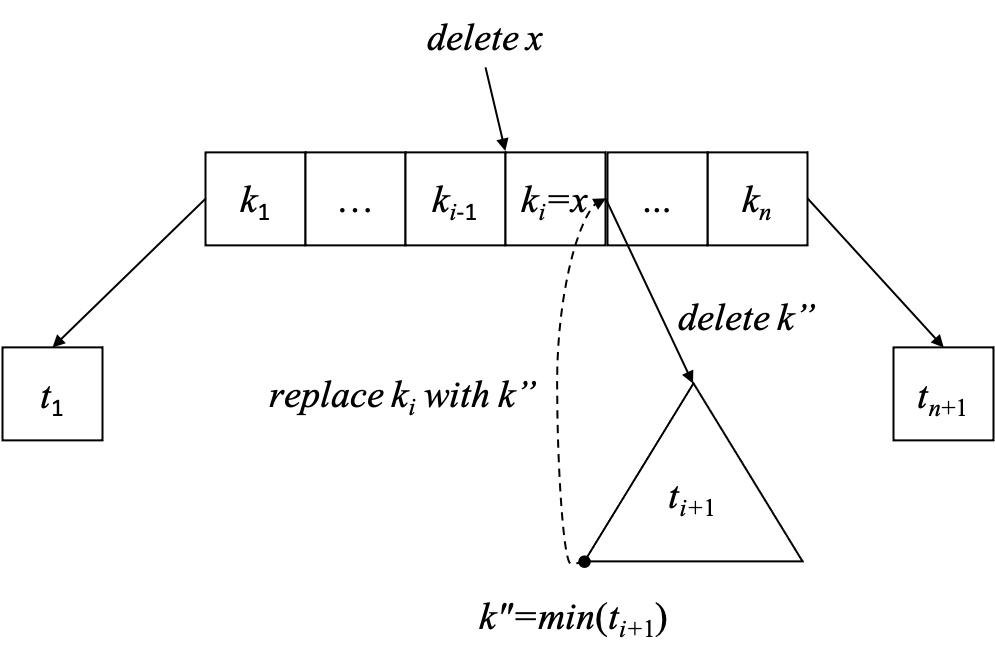
\includegraphics[scale=0.5]{img/btree-del-case2b.eps}
    \caption{Replace and delete from successor.} \label{fig:btree-del-case2b}
\end{figure}

\item Case 2c, Otherwise, if neither $y$, nor $z$ contains enough keys, we
can merge $y$, $k$ and $z$ into one new node, so that this new node
contains $2t-1$ keys. After that, we can then recursively do the removing.

Note that after merge, if the current node doesn't contain any keys,
which means $k$ is the only key in $x$. $y$ and $z$ are the only two
children of $x$. we need shrink the tree height by one.
\end{itemize}

Figure \ref{fig:btree-del-case2c} illustrates this sub-case.

\begin{figure}[htbp]
  \centering
    \includegraphics[scale=0.5]{img/btree-del-case2c.eps}
    \caption{Merge and delete.} \label{fig:btree-del-case2c}
\end{figure}

the last case states that, if $k$ can't be located in node $x$, the algorithm
need find a child node $c_i$ in $x$, so that the sub-tree $c_i$
contains $k$. Before the deletion is recursively applied in $c_i$, we
need make sure that there are at least $t$ keys in $c_i$. If there are
not enough keys, the following adjustment is performed.

\begin{itemize}
\item Case 3a, We check the two sibling of $c_i$, which are $c_{i-1}$ and $c_{i+1}$.
If either one contains enough keys (at least $t$ keys), we move
one key from $x$ down to $c_i$, and move one key from the sibling up to
$x$. Also we need move the relative child from the sibling to $c_i$.

This operation makes $c_i$ contains enough keys for deletion. we can
next try to delete $k$ from $c_i$ recursively.

Figure \ref{fig:btree-del-case3a} illustrates this case.

\begin{figure}[htbp]
  \centering
    \includegraphics[scale=0.5]{img/btree-del-case3a.eps}
    \caption{Borrow from the right sibling.}
    \label{fig:btree-del-case3a}
\end{figure}

\item Case 3b, In case neither one of the two siblings contains enough keys, we then
merge $c_i$, a key from $x$, and either one of the sibling into a new
node. Then do the deletion on this new node.
\end{itemize}

Figure \ref{fig:btree-del-case3b} shows this case.

\begin{figure}[htbp]
  \centering
    \includegraphics[scale=0.5]{img/btree-del-case3b.eps}
    \caption{Merge $c_i$, $k$, and $c_{i+1}$ to a new node.}
    \label{fig:btree-del-case3b}
\end{figure}

Before define the B-tree delete algorithm, we need provide some auxiliary
functions. Function \textproc{Can-Del} tests if a node contains enough keys
for deletion.

\begin{algorithmic}[1]
\Function{Can-Del}{$T$}
  \State \Return $|K(T)| \ge t$
\EndFunction
\end{algorithmic}

Procedure \textproc{Merge-Children}($T, i$) merges child $c_i(T)$, key $k_i(T)$,
and child $c_{i+1}(T)$ into one big node.

\begin{algorithmic}[1]
\Procedure{Merge-Children}{$T, i$} \Comment{Merge $c_i(T)$, $k_i(T)$, and $c_{i+1}(T)$}
  \State $x \gets c_i(T)$
  \State $y \gets c_{i+1}(T)$
  \State $K(x) \gets K(x) \cup \{k_i(T)\} \cup K(y)$
  \State $C(x) \gets C(x) \cup C(y)$
  \State \Call{Remove-At}{$K(T), i$}
  \State \Call{Remove-At}{$C(T), i+1$}
\EndProcedure
\end{algorithmic}

Procedure \textproc{Merge-Children} merges the $i$-th child, the $i$-th key,
and $i+1$-th child of node $T$ into a new child, and remove the
$i$-th key and $i+1$-th child from $T$ after merging.

With these functions defined, the B-tree deletion algorithm can be given by
realizing the above 3 cases.

\begin{algorithmic}[1]
\Function{Delete}{$T, k$}
  \State $i \gets 1$
  \While{$i \leq |K(T)|$}
    \If{$k = k_i(T)$}
      \If{$T$ is leaf} \Comment{case 1}
        \State \Call{Remove}{$K(T), k$}
      \Else \Comment{case 2}
        \If{\Call{Can-Del}{$c_i(T)$}} \Comment{case 2a}
          \State $k_i(T) \gets$ \Call{Last-Key}{$c_i(T)$}
          \State \Call{Delete}{$c_i(T), k_i(T)$}
        \ElsIf{\Call{Can-Del}{$c_{i+1}(T)$}} \Comment{case 2b}
          \State $k_i(T) \gets$ \Call{First-Key}{$c_{i+1}(T)$}
          \State \Call{Delete}{$c_{i+1}(T), k_i(T)$}
        \Else \Comment{case 2c}
          \State \Call{Merge-Children}{$T, i$}
          \State \Call{Delete}{$c_i(T), k$}
          \If{$K(T) = NIL$}
            \State $T \gets c_i(T)$ \Comment{Shrinks height}
          \EndIf
        \EndIf
      \EndIf
      \State \Return $T$
    \ElsIf{$k < k_i(T)$}
      \State Break
    \Else
      \State $i \gets i+1$
    \EndIf
  \EndWhile
  \Statex
  \If{$T$ is leaf}
    \State \Return $T$ \Comment{$k$ doesn't exist in $T$.}
  \EndIf
  \If{$\lnot$ \Call{Can-Del}{$c_i(T)$}}  \Comment{case 3}
    \If{$i>1 \land$ \Call{Can-Del}{$c_{i-1}(T)$}} \Comment{case 3a: left sibling}
      \State \Call{Insert}{$K(c_i(T)), k_{i-1}(T)$}
      \State $k_{i-1}(T) \gets$ \Call{Pop-Back}{$K(c_{i-1}(T))$}
      \If{$c_i(T)$ isn't leaf}
        \State $c \gets$ \Call{Pop-Back}{$C(c_{i-1}(T))$}
        \State \Call{Insert}{$C(c_i(T)), c$}
      \EndIf
    \ElsIf{$i \leq |C(T)| \land$ \Call{Can-Del}{$c_{i_1}(T)$}} \Comment{case 3a: right sibling}
      \State \Call{Append}{$K(c_i(T)), k_i(T)$}
      \State $k_i(T) \gets$ \Call{Pop-Front}{$K(c_{i+1}(T))$}
      \If{$c_i(T)$ isn't leaf}
        \State $c \gets$ \Call{Pop-Front}{$C(c_{i+1}(T))$}
        \State \Call{Append}{$C(c_i(T)), c$}
      \EndIf
    \Else \Comment{case 3b}
      \If{$i>1$}
        \State \Call{Merge-Children}{$T, i-1$}
      \Else
        \State \Call{Merge-Children}{$T, i$}
      \EndIf
    \EndIf
  \EndIf
  \State \Call{Delete}{$c_i(T), k$} \Comment {recursive delete}
  \If{$K(T) = NIL$} \Comment {Shrinks height}
    \State $T \gets c_1(T)$
  \EndIf
  \State \Return $T$
\EndFunction
\end{algorithmic}

Figure \ref{fig:result-del1}, \ref{fig:result-del2}, and \ref{fig:result-del3}
show the deleting process step by step. The nodes modified are shaded.

\begin{figure}[htbp]
  \centering
  \subcaptionbox{A B-tree before deleting.}{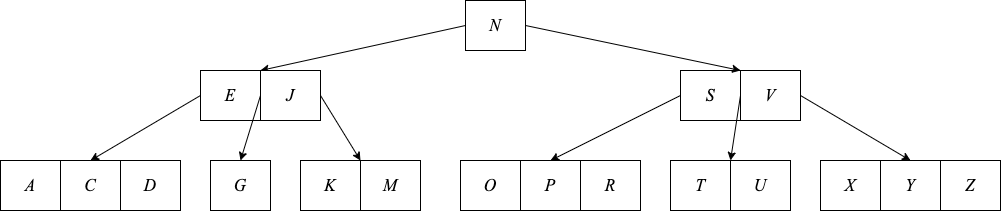
\includegraphics[scale=0.5]{img/btree-del-before.ps}} \\
  \subcaptionbox{After delete key 'F', case 1.}{\includegraphics[scale=0.5]{img/btree-del-F.ps}}
  \caption{Result of B-tree deleting (1).} \label{fig:result-del1}
\end{figure}

\begin{figure}[htbp]
  \centering
  \subcaptionbox{After delete key 'M', case 2a.}{\includegraphics[scale=0.5]{img/btree-del-M.ps}} \\
  \subcaptionbox{After delete key 'G', case 2c.}{\includegraphics[scale=0.5]{img/btree-del-G.ps}}
  \caption{Result of B-tree deleting program (2)} \label{fig:result-del2}
\end{figure}

\begin{figure}[htbp]
  \centering
  \subcaptionbox{After delete key 'D', case 3b, and height is shrunk.}{\includegraphics[scale=0.5]{img/btree-del-D.ps}} \\
  \subcaptionbox{After delete key 'B', case 3a, borrow from right sibling.}{\includegraphics[scale=0.5]{img/btree-del-B.ps}} \\
  \subcaptionbox{After delete key 'U', case 3a, borrow from left sibling.}{\includegraphics[scale=0.5]{img/btree-del-U.ps}}
  \caption{Result of B-tree deleting program (3)} \label{fig:result-del3}
\end{figure}

The following example Python program implements the B-tree deletion algorithm.

\lstset{language=Python}
\begin{lstlisting}
def can_remove(tr):
    return len(tr.keys) >= tr.t

def replace_key(tr, i, k):
    tr.keys[i] = k
    return k

def merge_children(tr, i):
    tr.children[i].keys += [tr.keys[i]] + tr.children[i+1].keys
    tr.children[i].children += tr.children[i+1].children
    tr.keys.pop(i)
    tr.children.pop(i+1)

def B_tree_delete(tr, key):
    i = len(tr.keys)
    while i>0:
        if key == tr.keys[i-1]:
            if tr.leaf:  # case 1 in CLRS
                tr.keys.remove(key)
            else: # case 2 in CLRS
                if tr.children[i-1].can_remove(): # case 2a
                    key = tr.replace_key(i-1, tr.children[i-1].keys[-1])
                    B_tree_delete(tr.children[i-1], key)
                elif tr.children[i].can_remove(): # case 2b
                    key = tr.replace_key(i-1, tr.children[i].keys[0])
                    B_tree_delete(tr.children[i], key)
                else: # case 2c
                    tr.merge_children(i-1)
                    B_tree_delete(tr.children[i-1], key)
                    if tr.keys==[]: # tree shrinks in height
                        tr = tr.children[i-1]
            return tr
        elif key > tr.keys[i-1]:
            break
        else:
            i = i-1
    # case 3
    if tr.leaf:
        return tr #key doesn't exist at all
    if not tr.children[i].can_remove():
        if i>0 and tr.children[i-1].can_remove(): #left sibling
            tr.children[i].keys.insert(0, tr.keys[i-1])
            tr.keys[i-1] = tr.children[i-1].keys.pop()
            if not tr.children[i].leaf:
                tr.children[i].children.insert(0, tr.children[i-1].children.pop())
        elif i<len(tr.children) and tr.children[i+1].can_remove(): #right sibling
            tr.children[i].keys.append(tr.keys[i])
            tr.keys[i]=tr.children[i+1].keys.pop(0)
            if not tr.children[i].leaf:
                tr.children[i].children.append(tr.children[i+1].children.pop(0))
        else: # case 3b
            if i>0:
                tr.merge_children(i-1)
            else:
                tr.merge_children(i)
    B_tree_delete(tr.children[i], key)
    if tr.keys==[]: # tree shrinks in height
        tr = tr.children[0]
    return tr
\end{lstlisting}

% ================================================================
%               Delete and fix method
% ================================================================

\subsection{Delete and fix method}

The merge and delete algorithm is a bit complex.
There are several cases, and in each case, there are sub cases to deal.

Another approach to design the deleting algorithm is to perform fixing
after deletion. It is similar to the insert-then-fix strategy.

\be
delete(T, k) = fix(del(T, k))
\ee

When delete a key from B-tree, we firstly locate
which node this key is contained. We traverse
from the root to the leaves till find this key in some node.

If this node is a leaf, we can remove the key, and then
examine if the deletion makes the node contains too few keys to
satisfy the B-tree balance properties.

If it is a branch node, removing the key breaks the node into
two parts. We need merge them together. The merging is a recursive
process which is shown in figure \ref{fig:del-fp-merge}.

\begin{figure}[htbp]
  \centering
  \includegraphics[scale=0.5]{img/btree-del-fp-merge.eps}
  \caption{Delete a key from a branch node. Removing $k_i$ breaks
the node into 2 parts. Merging these 2 parts
is a recursive process. When the two parts are leaves, the merging
terminates.} \label{fig:del-fp-merge}
\end{figure}

When do merging, if the two nodes are not leaves, we merge the keys
together, and recursively merge the last child of the left part
and the first child of the right part to one new node. Otherwise,
if they are leaves, we merely put all keys together.

Till now, the deleting is performed in straightforward way. However, deleting
decreases the number of keys of a node, and it may result in
violating the B-tree balance properties. The solution is to perform
fixing along the path traversed from root.

\begin{figure}[htbp]
  \centering
  \includegraphics[scale=0.5]{img/btree-del-fp-make.eps}
  \caption{After delete key $k$ from node $c_i$, denote the result
as $c_i'$. The fixing makes a new node from the
left part, $c_i'$ and the right part.}
  \label{fig:del-fp-make}
\end{figure}

During the recursive deletion, the branch node is broken into 3 parts.
The left part contains all keys less than $k$, includes $k_1, k_2, ..., k_{i-1}$,
and children $c_1, c_2, ..., c_{i-1}$, the right part contains all keys
greater than $k$, say $k_i, k_{i+1}, ..., k_{n+1}$, and children
$c_{i+1}, c_{i+2}, ..., c_{n+1}$. Then key $k$ is recursively deleted
from child $c_i$. Denote the result becomes $c_i'$ after that.
We need make a new node from these 3 parts,
as shown in figure \ref{fig:del-fp-make}.

At this time point, we need examine if $c_i'$ contains enough keys.
If there are too less keys (less than $t-1$, but not $t$ in
contrast to the merge-and-delete approach), we can either borrow a key-child
pair from the left or the right part, and do inverse operation of
splitting. Figure \ref{fig:del-fp-fixlow} shows example of borrowing from the left part.

\begin{figure}[htbp]
  \centering
  \includegraphics[scale=0.5]{img/btree-del-fp-fixlow.eps}
  \caption{Borrow a key-child pair from left part and
un-split to a new child.} \label{fig:del-fp-fixlow}
\end{figure}

If both left part and right part are empty, we can simply
push $c_i'$ up.

Denote the B-tree as $T=(K, C, t)$, where $K$ and $C$ are keys and children.
The $del(T, k)$ function deletes key $k$
from the tree.

\be
del(T, k) = \left \{
  \begin{array}
  {r@{\quad:\quad}l}
  (delete(K, k), \phi, t) & C = \phi \\
  merge((K_1, C_1, t), (K_2, C_2, t)) & k_i = k \\
  make((K_1', C_1'), del(c, k), (K_2', C_2')) & k \notin K
  \end{array}
\right.
\ee

If children $C = \phi$ is empty, $T$ is leaf. $k$ is deleted from keys directly.
Otherwise, $T$ is internal node. If $k \in K$, removing it separates the keys
and children in two parts $(K_1, C_1)$ and $(K_2, C_2)$. They will be recursively
merged.

\[
\begin{array}{l}
K_1 = \{k_1, k_2, ..., k_{i-1}\} \\
K_2 = \{k_{i+1}, k_{i+2}, ..., k_m\} \\
C_1 = \{c_1, c_2, ..., c_i\} \\
C_2 = \{c_{i+1}, c_{i+2}, ..., c_{m+1}\}
\end{array}
\]

If $k \notin K$, we need locate a child $c$, and further delete $k$ from
it.

\[
\begin{array}{l}
(K_1', K_2') = (\{k' | k' \in K, k' < k \}, \{k' | k' \in K, k < k' \}) \\
(C_1', \{c\} \cup C_2') = splitAt(|K_1'|, C)
\end{array}
\]

The recursive merge function is defined as the following. When merge two
trees $T_1 = (K_1, C_1, t)$ and $T_2 = (K_2, C_2, t)$, if both are leaves,
we create a new leave by concatenating the keys. Otherwise, the last
child in $C_1$, and the first child in $C_2$ are recursively merged.
And we call $make$ function to form the new tree. When $C_1$ and $C_2$
are not empty, denote the last child of $C_1$ as $c_{1, m}$, the rest
as $C_1'$; the first child of $C_2$ as $C_{2, 1}$, the rest as $C_2'$.
Below equation defines the merge function.

\be
merge(T_1, T_2) = \left \{
  \begin{array}
  {r@{\quad:\quad}l}
  (K_1 \cup K_2, \phi, t) & C_1 = C_2 = \phi \\
  make((K_1, C_1'), merge(c_{1,m}, c_{2, 1}), (K_2, C_2')) & otherwise
  \end{array}
\right.
\ee

The $make$ function defined above only handles the case that a node
contains too many keys due to insertion. When delete key, it may
cause a node contains too few keys. We need test and fix this
situation as well.

\be
make((K', C'), c, (K'', C'')) = \left \{
  \begin{array}
  {r@{\quad:\quad}l}
  fixFull((K', C'), c, (K'', C'')) & full(c) \\
  fixLow((K', C'), c, (K'', C'')) & low(c) \\
  (K' \cup K'', C' \cup \{c\} \cup C'', t) & otherwise
  \end{array}
\right.
\ee

Where $low(T)$ checks if there are too few keys less than $t-1$.
Function $fixLow(P_l, c, P_r)$ takes three arguments, the left pair of keys and children,
a child node, and the right pair of keys and children.
If the left part isn't empty, we borrow a pair of key-child, and
do un-splitting to make the child contain enough keys, then recursively
call $make$; If the right part isn't empty, we borrow a pair
from the right; and if both sides are empty, we
return the child node as result. In this case, the height of the tree
shrinks.

Denote the left part $P_l = (K_l, C_l)$. If $K_l$ isn't empty, the last
key and child are represented as $k_{l, m}$ and $c_{l, m}$ respectively.
The rest keys and children become $K_l'$ and $C_l'$; Similarly, the
right part is denoted as $P_r = (K_r, C_r)$. If $K_r$ isn't empty, the
first key and child are represented as $k_{r, 1}$, and $c_{r, 1}$. The
rest keys and children are $K_r'$ and $C_r'$. Below equation gives
the definition of $fixLow$.

\be
fixLow(P_l, c, P_r) = \left \{
  \begin{array}
  {r@{\quad:\quad}l}
  make((K_l', C_l'), unsplit(c_{l, m}, k_{l, m}, c), (K_r, C_r)) & K_l \neq \phi \\
  make((K_r, C_r), unsplit(c, k_{r, 1}, c_{r, 1}), (K_r', C_r')) & K_r \neq \phi \\
  c & otherwise
  \end{array}
\right.
\ee

Function $unsplit(T_1, k, T_2)$ is the inverse operation to splitting.
It forms a new B-tree nodes from two small nodes and a key.

\be
unsplit(T_1, k, T_2) = (K_1 \cup \{k\} \cup K_2, C_1 \cup C_2, t)
\ee

The following example Haskell program implements the B-tree deletion
algorithm.

\lstset{language=Haskell}
\begin{lstlisting}
import qualified Data.List as L

delete tr x = fixRoot $ del tr x

del:: (Ord a) => BTree a -> a -> BTree a
del (Node ks [] t) x = Node (L.delete x ks) [] t
del (Node ks cs t) x =
    case L.elemIndex x ks of
      Just i -> merge (Node (take i ks) (take (i+1) cs) t)
                      (Node (drop (i+1) ks) (drop (i+1) cs) t)
      Nothing -> make (ks', cs') (del c x) (ks'', cs'')
    where
      (ks', ks'') = L.partition (<x) ks
      (cs', (c:cs'')) = L.splitAt (length ks') cs

merge (Node ks [] t) (Node ks' [] _) = Node (ks++ks') [] t
merge (Node ks cs t) (Node ks' cs' _) = make (ks, init cs)
                                             (merge (last cs) (head cs'))
                                             (ks', tail cs')

make (ks', cs') c (ks'', cs'')
    | full c = fixFull (ks', cs') c (ks'', cs'')
    | low c  = fixLow  (ks', cs') c (ks'', cs'')
    | otherwise = Node (ks'++ks'') (cs'++[c]++cs'') (degree c)

low tr = (length $ keys tr) < (degree tr)-1

fixLow (ks'@(_:_), cs') c (ks'', cs'') = make (init ks', init cs')
                                              (unsplit (last cs') (last ks') c)
                                              (ks'', cs'')
fixLow (ks', cs') c (ks''@(_:_), cs'') = make (ks', cs')
                                              (unsplit c (head ks'') (head cs''))
                                              (tail ks'', tail cs'')
fixLow _ c _ = c

unsplit c1 k c2 = Node ((keys c1)++[k]++(keys c2))
                       ((children c1)++(children c2)) (degree c1)
\end{lstlisting}

When delete the same keys from the B-tree as in delete and fixing
approach, the results are different. However, both satisfy
the B-tree properties, so they are all valid.

\begin{figure}[htbp]
  \centering
  \subcaptionbox{B-tree before deleting}{\includegraphics[scale=0.5]{img/btree-del-fp-before.ps}}\\
  \subcaptionbox{After delete key 'E'.}{\includegraphics[scale=0.5]{img/btree-del-fp-E.ps}}
  \caption{Result of delete-then-fixing (1)} \label{fig:result-del-fp1}
\end{figure}

\begin{figure}[htbp]
  \centering
  \subcaptionbox{After delete key 'G',}{\includegraphics[scale=0.5]{img/btree-del-fp-G.ps}} \\
  \subcaptionbox{After delete key 'A'.}{\includegraphics[scale=0.5]{img/btree-del-fp-A.ps}}
  \caption{Result of delete-then-fixing (2)} \label{fig:result-del-fp2}
\end{figure}

\begin{figure}[htbp]
  \centering
  \subcaptionbox{After delete key 'M'.}{\includegraphics[scale=0.5]{img/btree-del-fp-M.ps}} \\
  \subcaptionbox{After delete key 'U'.}{\includegraphics[scale=0.5]{img/btree-del-fp-U.ps}}
  \caption{Result of delete-then-fixing (3)} \label{fig:result-del-fp3}
\end{figure}


% ================================================================
%               Searching
% ================================================================
\section{Searching}
\index{B-tree!search}

Searching in B-tree can be considered as the generalized
tree search extended from binary search tree.

When searching in the binary tree, there are only 2 different directions,
the left and the right. However, there are multiple directions in B-tree.

\begin{algorithmic}[1]
\Function{Search}{$T, k$}
  \Loop
    \State $i \gets 1$
    \While{$i \leq |K(T)| \land k > k_i(T)$}
      \State $i \gets i+1$
    \EndWhile
    \If{$i \leq |K(T)| \land k = k_i(T)$}
      \State \Return $(T, i)$
    \EndIf
    \If{$T$ is leaf}
      \State \Return $NIL$ \Comment{$k$ doesn't exist}
    \Else
      \State $T \gets c_i(T)$
    \EndIf
  \EndLoop
\EndFunction
\end{algorithmic}

Starts from the root, this program examines each key one by one
from the smallest to the biggest. In case it finds the
matched key, it returns the current node and the index of this
key. Otherwise, if it finds the position $i$ that $k_i < k < k_{i+1}$,
the program will next search the child node
$c_{i+1}$ for the key. If it traverses to some leaf node, and
fails to find the key, the empty value is returned to
indicate that this key doesn't exist in the tree.

The following example Python program implements the search algorithm.

\lstset{language=Python}
\begin{lstlisting}
def B_tree_search(tr, key):
    while True:
        for i in range(len(tr.keys)):
            if key <= tr.keys[i]:
                break
        if key == tr.keys[i]:
            return (tr, i)
        if tr.leaf:
            return None
        else:
            if key > tr.keys[-1]:
                i=i+1
            tr = tr.children[i]
\end{lstlisting}

The search algorithm can also be realized by recursion. When search
key $k$ in B-tree $T = (K, C, t)$, we partition the keys with $k$.

\[
\begin{array}{l}
K_1 = \{ k' | k' < k \} \\
K_2 = \{ k' | k \leq k' \}
\end{array}
\]

Thus $K_1$ contains all the keys less than $k$, and $K_2$ holds the
rest. If the first element in $K_2$ is equal to $k$, we find the key.
Otherwise, we recursively search the key in child $c_{|K_1|+1}$.

\be
search(T, k) = \left \{
  \begin{array}
  {r@{\quad:\quad}l}
  (T, |K_1|+1) & k \in K_2 \\
  \phi & C = \phi \\
  search(c_{|K_1|+1}, k) & otherwise
  \end{array}
\right.
\ee

Below example Haskell program implements this algorithm.

\lstset{language=Haskell}
\begin{lstlisting}
search :: (Ord a)=> BTree a -> a -> Maybe (BTree a, Int)
search tr@(Node ks cs _) k
    | matchFirst k $ drop len ks = Just (tr, len)
    | otherwise = if null cs then Nothing
                  else search (cs !! len) k
    where
      matchFirst x (y:_) = x==y
      matchFirst x _ = False
      len = length $ filter (<k) ks
\end{lstlisting}


% ================================================================
%                 Short summary
% ================================================================
\section{Notes and short summary}
In this chapter, we explained the B-tree data structure as a kind of
extension from binary search tree. The background knowledge of
magnetic disk access is skipped, user can refer to \cite{CLRS}
for detail. For the three main operations, insertion, deletion,
and searching, both imperative and functional algorithms are
given. They traverse from the root to the leaf. All the three
operations perform in time proportion to the height of the tree.
Because B-tree always maintains the balance properties. The
performance is ensured to bound to $O(\lg n)$ time,
where $n$ is the number of the keys in B-tree.

\begin{Exercise}
\begin{itemize}
\item When insert a key, we need find a position, where all keys on the left are less than it, while all the others on the right are greater than it. Modify the algorithm so that the elements stored in B-tree only need support less-than and equality test.
\item We assume the element being inserted doesn't exist in the tree. Modify the algorithm so that duplicated elements can be stored in a linked-list.
\item Eliminate the recursion in imperative B-tree insertion algorithm.
\end{itemize}
\end{Exercise}

\section{Appendix: Example programs}

Definition of B-tree:

\begin{lstlisting}[language = Bourbaki]
data BTree<K, Int deg> {
    [K] keys
    [BTree<K>] subStrees;
}
\end{lstlisting}

Split node

\begin{lstlisting}[language = Bourbaki]
void split(BTree<K, deg> z, Int i) {
    var d = deg
    var x = z.subTrees[i]
    var y = BTree<K, deg>()
    y.keys = x.keys[d ...]
    x.keys = x.keys[ ... d - 1]
    if not isLeaf(x) {
      y.subTrees = x.subTrees[d ... ]
      x.subTrees = x.subTrees[... d]
    }
    z.keys.insert(i, x.keys[d - 1])
    z.subTrees.insert(i + 1, y)
}

Bool isLeaf(BTree<K, deg> t) = t.subTrees == []
\end{lstlisting}

Insert a key to B-tree:

\begin{lstlisting}[language = Bourbaki]
BTree<K, deg> insert(BTree<K, deg> tr, K key) {
    var root = tr
    if isFull(root) {
        var s = BTree<K, deg>()
        s.subTrees.insert(0, root)
        split(s, 0)
        root = s
    }
    return insertNonfull(root, key)
}
\end{lstlisting}

Insert a key to a non-full node.

\begin{lstlisting}[language = Bourbaki]
BTree<K, deg> insertNonfull(BTree<K, deg> tr, K key) {
    if isLeaf(tr) {
        orderedInsert(tr.keys, key)
    } else {
        Int i = length(tr.keys)
        while i > 0 and key < tr.keys[i - 1] {
            i = i - 1
        }
        if isFull(tr.subTrees[i]) {
            split(tr, i)
            if key > tr.keys[i] then i = i + 1
        }
        insertNonfull(tr.subTree[i], key)
    }
    return tr
}
\end{lstlisting}

Where \texttt{orderedInsert} inserts an element to an ordered list.

\begin{lstlisting}[language = Bourbaki]
void orderedInsert([K] lst, K x) {
    Int i = length(lst)
    lst.append(x)
    while i > 0 and lst[i] < lst[i-1] {
        (lst[i-1], lst[i]) = (lst[i], lst[i-1])
        i = i - 1
    }
}

Bool isFull(BTree<K, deg> x) = length(x.keys) >= 2 * deg - 1
\end{lstlisting}

\ifx\wholebook\relax \else
\begin{thebibliography}{99}

\bibitem{CLRS}
Thomas H. Cormen, Charles E. Leiserson, Ronald L. Rivest and Clifford Stein. ``Introduction to Algorithms, Second Edition''. The MIT Press, 2001. ISBN: 0262032937.

\bibitem{wiki-b-tree}
B-tree, Wikipedia. http://en.wikipedia.org/wiki/B-tree

\bibitem{okasaki-rbtree}
Chris Okasaki. ``FUNCTIONAL PEARLS Red-Black Trees in a Functional Setting''. J. Functional Programming. 1998

\end{thebibliography}

\expandafter\enddocument
\fi
